\documentclass{article}
\usepackage{graphicx}
\usepackage{hyperref}
\usepackage[a4paper, margin=1.25in]{geometry}
\usepackage{breakcites}
\usepackage{subcaption}
\usepackage{float}
\usepackage{textcomp}
\usepackage{amsmath}
\usepackage{textgreek}
\usepackage{authblk}
\usepackage{rotating}
\usepackage{booktabs}
\usepackage{longtable}
\usepackage{lineno}
\usepackage[
  style=numeric,
  citestyle=numeric-comp,
  backend=biber,
  doi=true,
  natbib=true,
  sorting=none
]{biblatex}

\addbibresource{library.bib}

\begin{document}

\title{A Global Picture of Food Insecurity and Hunger}

\author[1,2,*]{Matthew Cooper}
\author[2,3]{Benjamin Müller}
\author[4]{Carlo Cafiero}
\author[2,5]{Juan Carlos Laso}
\author[2,6]{Homi Kharas}

\affil[1]{T.H. Chan School of Public Health, Harvard University}
\affil[2]{The World Data Lab, Vienna, Austria}
\affil[3]{Department of Economics, Vienna University of Economics and Business}
\affil[4]{The Food and Agricultural Organization of the United Nations}
\affil[5]{The International Institute for Applied Systems Analysis}
\affil[6]{The Brookings Institute}
\affil[*]{Corresponding Author: mcooper@hsph.harvard.edu}

\maketitle
\begin{abstract}
We modeled levels of of food security at a subnational level from 2010 to 2030 using microdata from 77 countries collected by the FAO and Gallup World Poll for the Voices of the Hungry project.  We find significant heterogeneity in levels of food security around the world, ranging from parts of the global north with less than 1\% of the population food insecure to parts of the global south where as much as 3 out of 4 people are severely food insecure.  Examining global temporal trends, we find that food insecurity has been increasing over the past several years, but under middle-of-the-road assumptions for development and population change, food insecurity will decline throughout the 2020s.  This global decrease is largely driven by trends in South and East Asia, and some parts of the world, particularly sub-Saharan Africa, are projected to show increases in the prevalence of food insecurity throughout the next decade. This is the first global picture of the Food Insecurity Experience Scale, the food security metric most indicative of the lived experience of hunger.
\end{abstract}

\section{Introduction}
Being food secure is a critical component of human flourishing, which is why the second Sustainable Development Goal (SDG2) is ``Zero Hunger".  While a number of indicators are used to track progress towards this goal, the indicator that is most indicative of the human experience of food insecurity is the Food Insecurity Experience Scale, or FIES.  The FIES was developed due to a recognized need to measure actual food insecurity based on personal exposure to hunger, rather than proxies for food insecurity, such as estimates of calories per capita, or health consequences of food insecurity, such as child stunting.  However, as a relatively new metric, little work has been done so far to model food security at a global scale or estimate current trends in the number of food insecure people using the FIES.

Food security has traditionally been difficult to measure, and this has led to incomplete or inaccurate pictures of global hunger.  Metrics of macro-health, such as anthropometry and mortality rates are correlated broadly with food insecurity and have been used for many years to monitor human well-being \citep{Puffer1973, Habicht1974}.  However, these metrics are confounded with other determinants of health such as infectious disease and are not meaningful at the scale of individuals or households \citep{Perumal2018}.  Other proxies for food security, such as food availability estimated from crop yields \citep{Maxwell1992}, are also inadequate because they do not indicate how accessible food is to the general population, and food insecurity can certainly occur in the absence of food availability decline \citep{Sen1983}.  Moreover, these metrics are very sensitive to incorrect estimates of crop yields and food reserves at a national scale.  Thus, global estimates of hunger and food insecurity based on these metrics carry forward similar flaws.

As researchers began to focus on food insecurity at the individual and household level, household microdata collecting information on household finances and consumption became a common proxy for food security \citep{Haddad1994}.  However, these efforts were criticized for being onerous, insufficiently comparable, as well as for ignoring subjective and experiential aspects of food security \citep{Maxwell1996}.  This led to the emergence of several indicators designed to be rapidly deployable, culturally cross-comparable, and based on the lived experience of food security \citep{Jones2013}.  These metrics include the Household Food Insecurity and Access Scale (HFIAS) \citep{Coates2007}; the Coping Strategies Index (CSI) \citep{Maxwell1999}; and the Household Hunger Scale (HHS) \citep{Ballard2011}.

Drawing on the insights derived in designing and implementing these novel food security metrics, the FIES was developed by the Food and Agricultural Organization (FAO) of the UN \cite{Ballard2013}.  The FIES is based on a survey of eight behaviors indicative of food insecurity and hunger over the previous year, such as skipping meals or worrying about having enough to eat.  Using a Rash model \citep{Cafiero2018}, each individual in the survey is given a severity score, and thresholds for moderate and severe food insecurity are set at the behaviors of eating less than the respondent thought they should, and not eating for a while day, respectively.  Thus, people in moderate-to-severe food insecurity are estimated to have not eaten as much as they should have at least once in the previous year, while people in severe food insecurity are estimated to have gone an entire day without eating in the previous year.

Since 2014, in partnership with Gallup World Poll, the FAO conducted surveys around the world in 77 countries and nearly 200 languages to estimate the prevalence of food insecurity using the FIES.  Using this data, we used machine learning to estimate levels of food insecurity around the world at the subnational level.  Our analysis highlights several important global and regional trends in food security.

\section{Results}
\subsection{Spatial Distribution of Food Insecurity}
We found significant heterogeneities in the global distribution of severe food insecurity, estimated to be people who had to go an entire day without eating at least once in the previous year (See Fig. \ref{fig:map}).  For the year 2020, mainland sub-Saharan Africa is the continent with with the highest rates of severe food insecurity, with at least 15\% of people in severe food insecurity in at last one region in every country except Gabon and Equatorial Guinea.  Outside of Africa, serious pockets of severe food insecurity also occur in Venezuela, Syria, Papua New Guinea, Yemen, and Afghanistan.  In many large middle-income countries, severe food insecurity is also quite prevalent, with rates between 10-15\% in areas like northern Brazil, many central Asian and middle-eastern countries, and India and Indonesia.

The experience of at least moderate food insecurity, or eating less than one would prefer, is quite common in many parts of the world.  In 2020, it is quite common in Africa, south and southeast Asia, and parts of Latin America, where in many places over 50\% of the population experiences this degree of food insecurity.  Even in countries widely considered to be developed, such as Australia, the United States, and parts of eastern and southern Europe, moderate-to-severe food insecurity is as high as 10-15\%.  

\begin{figure}[H]
  \centering
  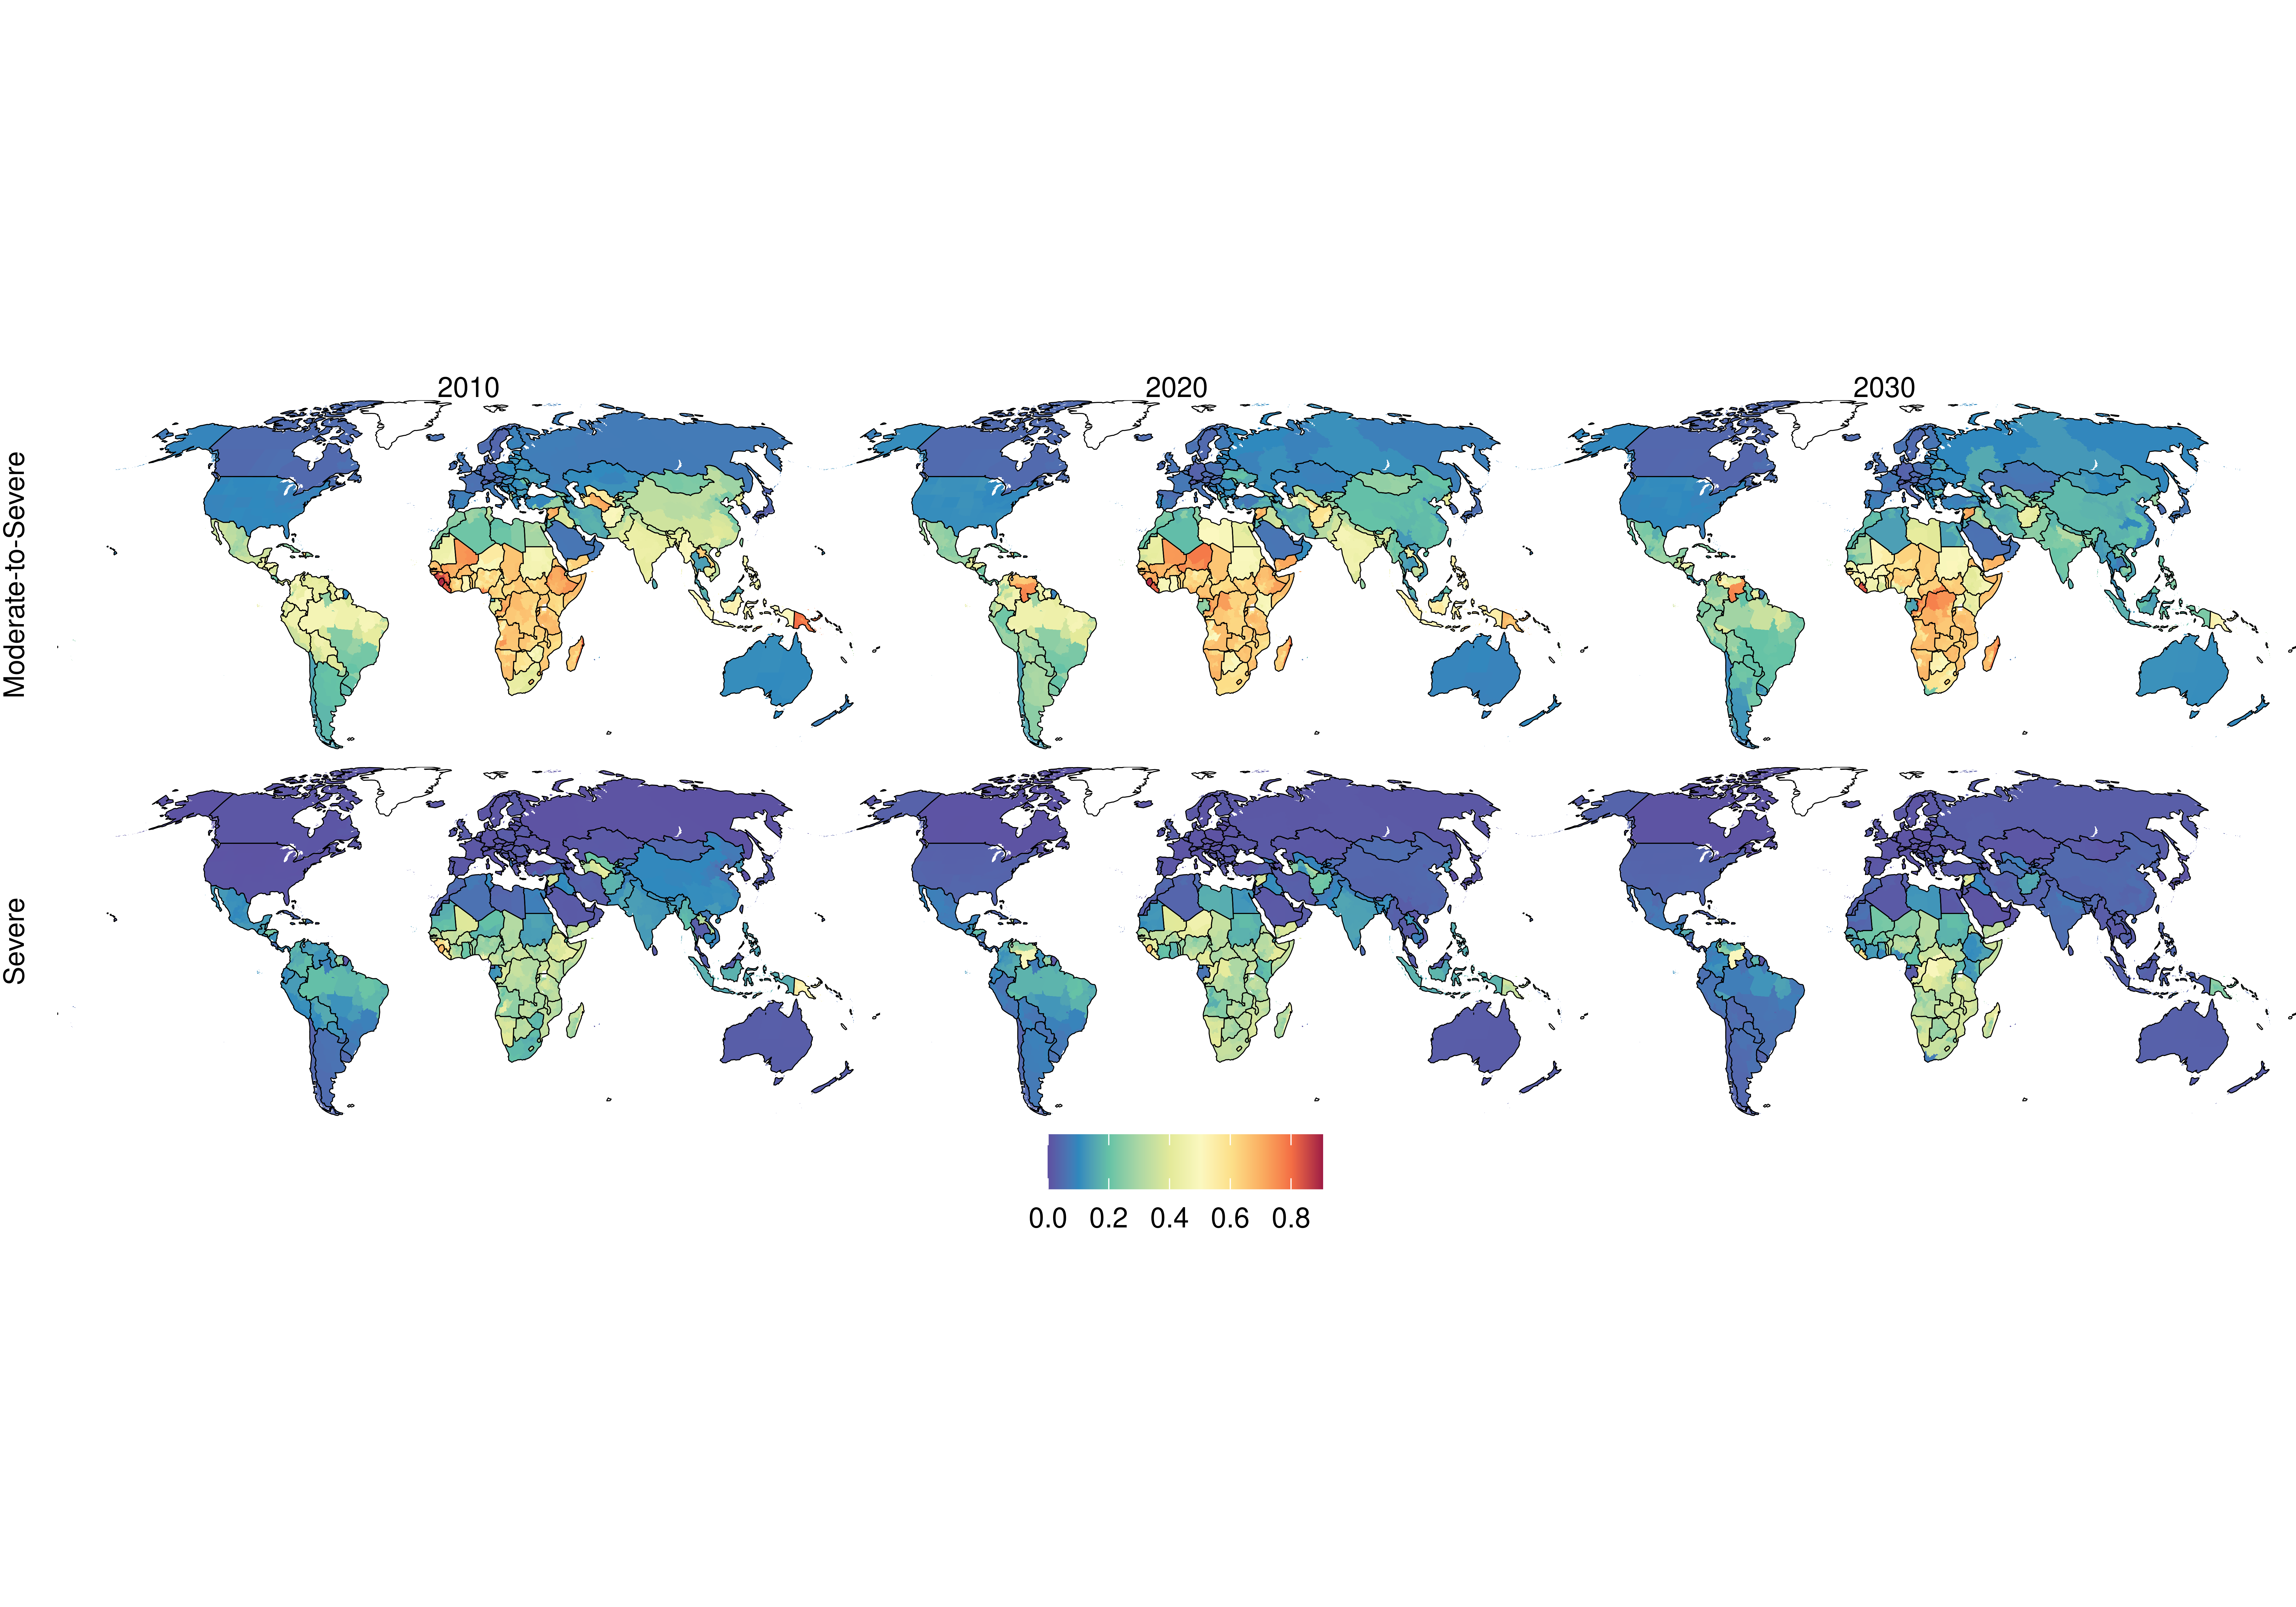
\includegraphics[width=\linewidth]{img/FullMap.pdf}
  \caption{Modeled rates of severe and moderate-to-severe food insecurity for the years 2010, 2020, and 2030}
  \label{fig:map}
\end{figure}

Globally, in the year 2020, we estimate that 2.33 billion people experience at least moderate food insecurity, and 829 million people experience severe food insecurity (See Fig. \ref{fig:timeseries}).  While the total number of people in moderate and severe food security held roughly constant for the 2010s and even increased in latter part of that decade, we predict that it will decline throughout the 2020s.  However, this overall decline will not be uniform across the world.  Our model expects that, in sub-Saharan Africa, moderate food insecurity will increase throughout the 2020s and severe food insecurity will plateau.  Food Security will fall in most other world regions, particularly South Asia and East Asia \& the Pacific.

\begin{figure}[H]
  \centering
  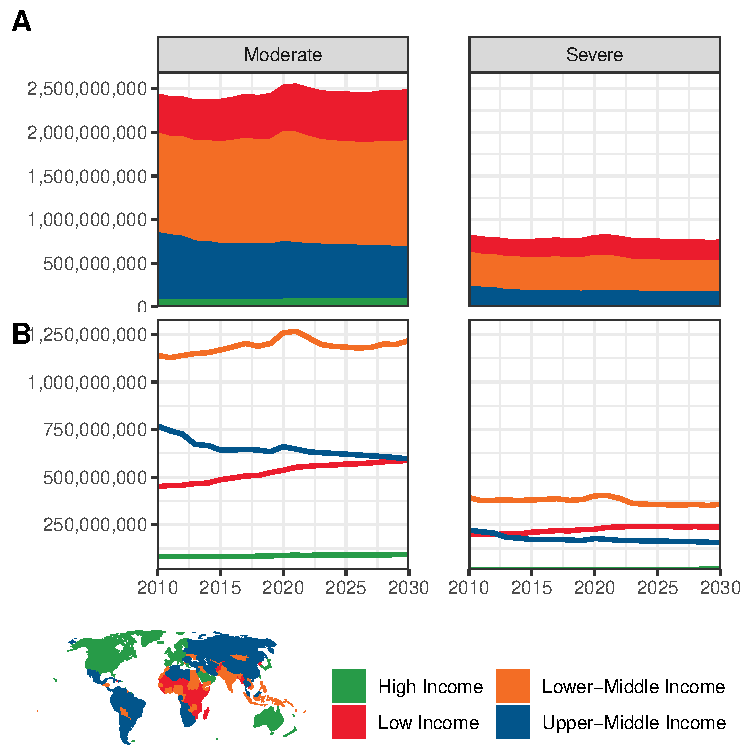
\includegraphics[width=\linewidth]{img/TimeSeries.pdf}
  \caption{Number of people in moderate-to-severe and severe food insecurity, by World Bank regions over time, with a 3-year smoothing.  Panel (A) shows the number of food insecure people with region totals stacked, to show global trends and totals over time.  Panel (B) shows regional totals compared against each other over time.}
  \label{fig:timeseries}
\end{figure}


\section{Discussion}
Compare with SOFI reports, other metrics of hunger.

Dynamics of population growth and development

Deal with scale - why modeling at admin1 is a different exercise than local level modeling

What is driving the increases?
What will drive the decreases? (caveats of RF method)

Next decade improvements in food insecurity will only fall like 10\%, not major in overall terms and nowhere near ambitious SDG target.

Cliamte change is not yet a major threat on a global scale, although there will be regional impacts

\section{Methods}

\subsection{Disaggregation}
The data on the FIES collected by Gallup 

Assumptions

\subsection{Covariates}

Selection and Processing

(Maybe put some in Appendix)

Cite determinants of FIES form \citep{smith2017world}.

\subsection{Modeling}

Random Forest

Hyperparameter selection

\section{Conclusion}

\printbibliography

\section*{Supplemental Info}
\setcounter{table}{0}
\setcounter{figure}{0}
\renewcommand{\thetable}{S\arabic{table}}
\renewcommand{\thefigure}{S\arabic{figure}}

\subsection{Component Questions of the FIES}
\begin{enumerate}
	\item During the last 12 MONTHS, was there a time when you were worried you would not have enough food to eat because of a lack of money or other resources?
	\item Still thinking about the last 12 MONTHS, was there a time when you were unable to eat healthy and nutritious food because of a lack of money or other resources?
	\item Was there a time when you ate only a few kinds of foods because of a lack of money or other resources?
- out-of-sample fit also very good, r2 around 0.99

- variable importance and coefficient table?

\section{Conclusion}

\printbibliography

\section*{Supplemental Info}
